\documentclass[11pt]{beamer}

\usepackage[utf8]{inputenc}
\usepackage[english]{babel}
\usepackage[font=tiny]{caption}
\usepackage{langsci-gb4e}

\setbeamerfont{subtitle}{size=\normalsize}
\setbeamerfont{title}{size=\Large}
\setbeamerfont{author}{size=\large}
\setbeamercovered{invisible}
\usepackage{xcolor}
\usepackage{mdframed}

\newenvironment{block*}{
    \begin{mdframed}[
        backgroundcolor=white,
        linecolor=black,
        linewidth=0pt,
        innerleftmargin=8pt,
        innerrightmargin=10pt,
        innertopmargin=6pt,
        innerbottommargin=6pt
    ]
}{
    \end{mdframed}
}

%make title, subtitle and presenter smaller
%impostazioni per la prima diapositiva
\title{{Tool use and language share syntactic processes and neural patterns in the basal ganglia}}

\subtitle{\small{\vspace*{0.2cm}by S. Thibault, R. Py, A. M. Gervasi, R. Salemme, E. Koun, M. Lövden, V. Boulenger, A. C. Roy, \& C. Brozzoli}}
\medskip

\author{\vspace*{-0.4cm}Presented by Gabriele De Leonardis}
\date{}

%impostazioni per la scelta di tema e colore 
\usetheme[cimec]{beunitn} 


%impostazioni per l'uso delle immagini
\usepackage{graphicx}
\graphicspath{{./images/paper_pics/}}
\usepackage[absolute, overlay]{textpos}

%impostazioni per l'uso di textblock
\usepackage[absolute, overlay]{textpos}

%setto il beamer a transparent per le altre scritte
\setbeamercovered{transparent}

%cambio l'ambiente matematico "teorema" in italiano
%\renewenvironment{proof}[1][Dimostrazione]{\noindent\textbf
%{#1.}}{\ \rule{0.5em}{0.5em}}
%\newtheorem{theorem}{Teorema}

%Permetto alla bibliografia di essere stampata anche se non citata
\nocite{*}

%costruzione della bibliografia
\usepackage{csquotes}
\usepackage[style=numeric]{biblatex}
\addbibresource{biblio.bib}


%\author{Gabriele De Leonardis}
%\date{}
\begin{document}
\begin{frame}[noframenumbering]
    \maketitle
\end{frame}

\section{Background}

\begin{frame}{Background}
%%%text
\setbeamercovered{invisible}

\fontsize{13pt}{16}\selectfont
\only<1-4>{
\vspace{-0.32cm}
\begin{columns}
\begin{column}{0.5\textwidth}
   \begin{itemize}
   \item Tool use adds \textbf{further hierarchical level} to the motor plan.
   \vspace{0.7cm}
   \pause
   \item Action and language \textbf{share syntactic processes}. Actions involve hierarchical interdependency within a motor sequence.
   \end{itemize}
\end{column}
\pause
\begin{column}{0.5\textwidth}  %%<--- here
    \begin{itemize}
        \item \textbf{Syntax} as the cognitive function handling \textbf{complex} linguistic \textbf{structures}.
        \vspace{0.7cm}
        \pause
        \item \textbf{Behavioral link} supported by neuroimaging.
    \end{itemize}
\end{column}
\end{columns}}
\pause
\only<5>{
\begin{itemize}
    \item \textbf{Syntactic} processing of hierarchical structures relies on activity within the \textbf{left IFG} and \textbf{BG}.
    \item Activity in the \textbf{BG} and \textbf{perietofrontal} network support skillful \textbf{tool use.}
\end{itemize}}

\end{frame}

%\input{1.1_Background}

%\input{1.2_Background}

%\input{1.3_Background}

%\input{1.4_Background}

%\input{1.5_Background}

\section{Questions}

\begin{frame}{Questions}
\setbeamercovered{invisible}
\textbf{\large Big Theoretical Question:} 
\begin{itemize}
    \item {\large How do humans process language in the brain?}
\end{itemize}
\pause

\bigskip


\invisible<1>{\textbf{\large Experimental Question:}
\begin{itemize}
    \item {\large Does tool use \textbf{share syntactic processes} with language?}
\end{itemize}}


\end{frame}

\section{Hypotheses}

\begin{frame}{Hypotheses}
\setbeamercovered{invisible}
\fontsize{11pt}{16}\selectfont
\begin{block}
{H$_1$ Experimental Hypothesis:} \begin{itemize}
    \item Tool use and syntax \textbf{share neural resources} and, as a consequence, that the two abilities \textbf{affect one another} at the behavioral level.
\end{itemize}
 \end{block}

\pause
\bigskip

\begin{block}
{H$_0$ Null Hypothesis:} \begin{itemize}
    \item Tool use \textbf{does not share} syntactic processes with language.
\end{itemize}
 \end{block}

\end{frame}

\section{Methods}

\begin{frame}{Methods}
\setbeamercovered{invisible}

\fontsize{11pt}{16}\selectfont
\begin{columns}
\begin{column}{0.5\textwidth}
{\large\textbf{Design:}}
\vspace{0.2cm}
\begin{itemize}
    \item 244 participants
    \item 5 different experiments
    \item Healthy, right-handed, French native
    \item No impairment
\end{itemize}

\end{column}
\begin{column}{0.5\textwidth}
\only<2>{
\begin{itemize}
    \item fMRI
    \item Behavioral tasks
\end{itemize}}
\end{column}
\end{columns}


\end{frame}

\section{Experiment 1}

\begin{frame}{Experiment 1}
\setbeamercovered{invisible}
\fontsize{11pt}{15}\selectfont

\only<1>{{\Large\textbf{Aim:}}\\
\vspace{0.2cm}
{\large\textbf{Anatomical overlap of tool use and syntactic activity in the BG}}

Used fMRI to map areas where syntactic processes and tool use overlap}
\pause
\only<2>{
\begin{center}
    {\Large\textbf{Experimental design:}}\\
    \vspace{1cm}
    {\Large 1$^{st}$ Task \hspace{2cm} 2$^{nd}$ Task}
\end{center}}
\pause
\only<3>{
\begin{center}
    {\Large\textbf{Experimental design:}}\\
    \vspace{1cm}
    {\Large\textbf{1$^{st}$ Task} \hspace{2cm} 2$^{nd}$ Task}
\end{center}}
\end{frame}




\begin{frame}{Experiment 1}
\setbeamercovered{invisible}
\fontsize{12pt}{15}\selectfont

{\large\textbf{1$^{st}$ Task:}}\\
\vspace{0.2cm}
\begin{itemize}
\item Sentences with \textbf{same content word}s but featuring \textbf{three different} syntactic structures:
    \begin{itemize}
        \item coordinated clause
        \item subject-related clause
        \item object-related clause
    \end{itemize}
\item Test affirmation $\rightarrow$ true or false wrt preceding sentence
\end{itemize}
\end{frame}

\begin{frame}{Experiment 1}
\setbeamercovered{invisible}
\vspace{-0.2cm}
%\begin{textblock*}{7cm}(3.7cm,4.6cm) % {block width} (coords)
\begin{figure}
    \centering
    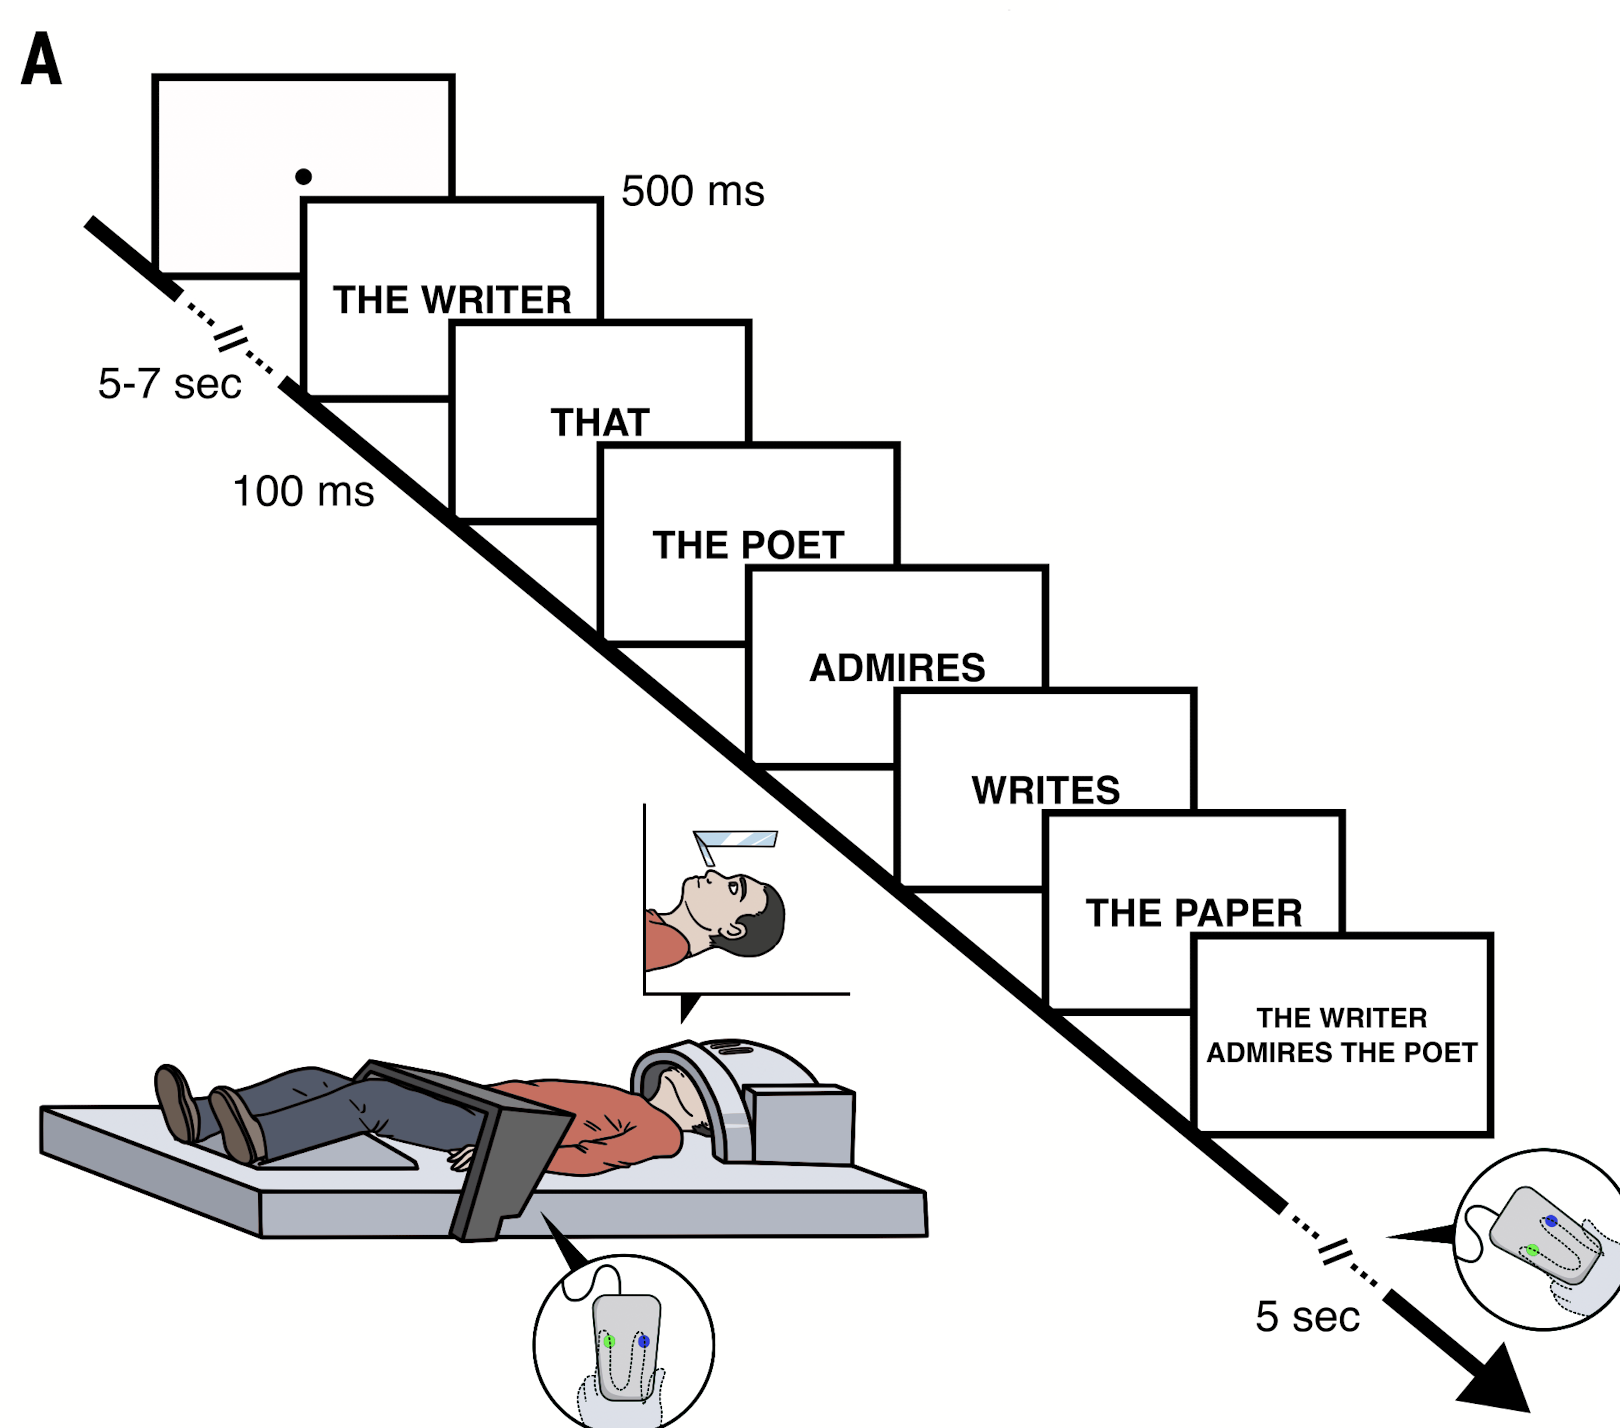
\includegraphics[width=8cm]{images/paper_pics/exp1.png}
    %\caption*{}
    \label{fig:label1}
\end{figure}

\end{frame}

\begin{frame}{Experiment 1}
\setbeamercovered{invisible}
\fontsize{12pt}{15}\selectfont
\vspace{-0.5cm}
{\Large\textbf{Results:}}\\
\vspace{0.2cm}

\only<1>{\begin{figure}
    \centering
    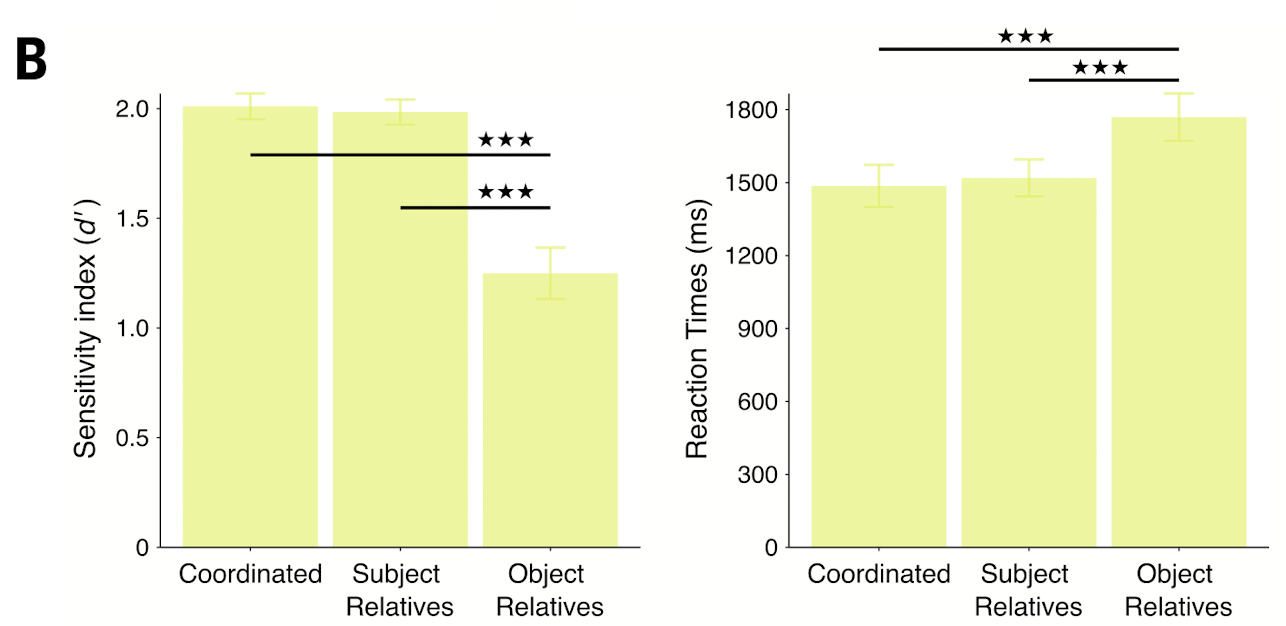
\includegraphics[width=8cm]{images/paper_pics/fig1B.png}
    \caption*{Object-relative clauses show worst sensitivity index scores and longest reaction time}
    \label{fig:label2}
\end{figure}}
\pause

\only<2>{\begin{itemize}\item \textbf{No difference} between subject-relative and coordinated clauses
\item $\rightarrow$ \textbf{Syntactic complexity} of the object relatives
\end{itemize}}
\pause
\only<3>{\begin{itemize} 
\item They assessed functional syntactic network by contrasting brain activation during object relatives vs the two other types of clauses.
\item Syntactic network: parietofrontal ensemble and BG (caudate nuclei, GPi, putamen). Left IFG also.
\end{itemize}}


\end{frame}

\begin{frame}{Experiment 1}
\setbeamercovered{invisible}
\fontsize{12pt}{15}\selectfont
\only<1>{
\begin{center}
    {\Large\textbf{Experimental design:}}\\
    \vspace{1cm}
    {\Large 1$^{st}$ Task \hspace{2cm} \textbf{2$^{nd}$ Task}}
\end{center}}
\pause
\only<2>{
{\large\textbf{2$^{nd}$ Task:}}\\
{\large\textbf{To capture the overlap of syntactic and tool-use networks}}
\begin{itemize}
\item Same participants were asked to use a pair of \textbf{pliers} or their free right hand
\item Had to \textbf{move a peg} from one side of a board to the other
\item Recorded brain activity and isolated portion about \textbf{tool movement planning}
\end{itemize}}
\pause
\only<3>{\begin{figure}
    \centering
    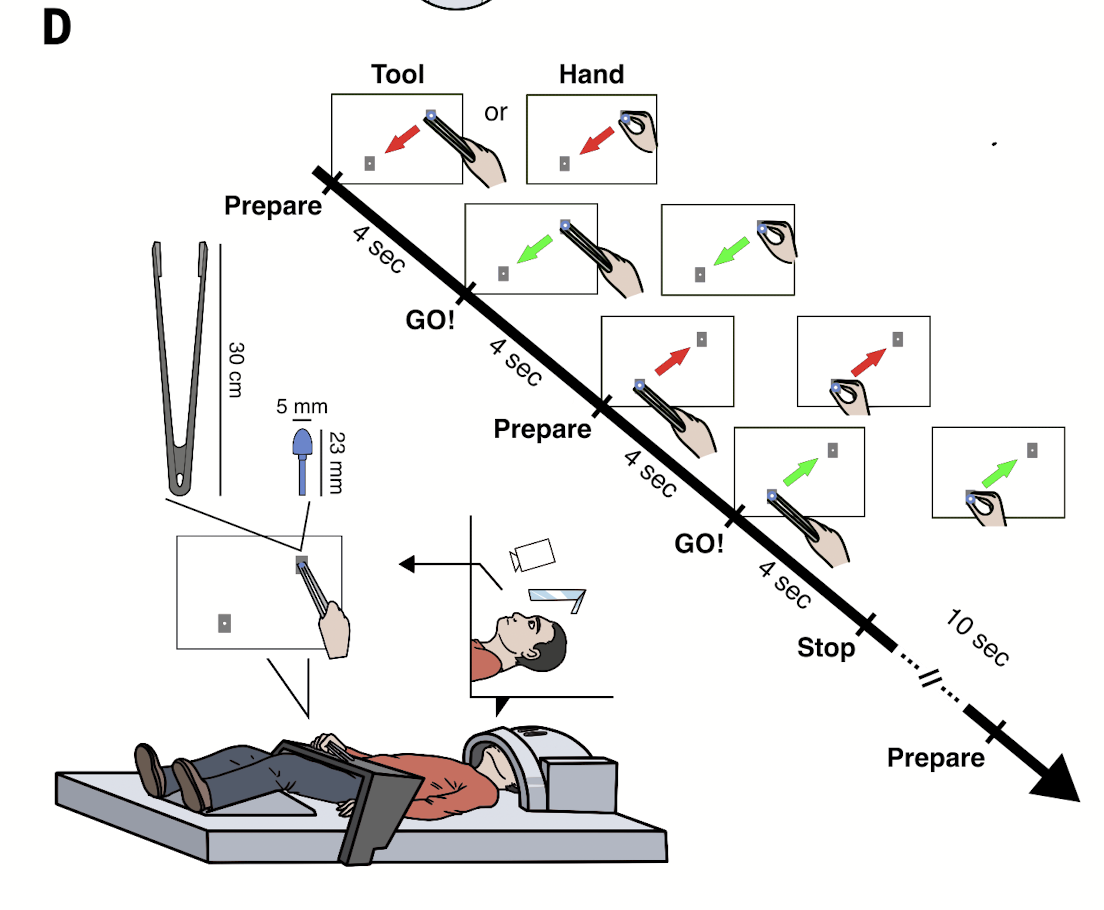
\includegraphics[width=8cm]{images/paper_pics/fig1D.png}
    %\caption*{}
    \label{fig:label3}
\end{figure}}
\pause
\only<4>{{\large\textbf{Results:}}
\begin{itemize}
    \item \textbf{Tool-use planning} found activation in parietal and prefrontal areas, and \textbf{BG} (both caudate nuclei, interbal globus pallidus, putamen). 
    \item Also ventral premotor cortex (within left IFG), though more posterior than findings for syntactic network.
\end{itemize}}

\end{frame}

\begin{frame}{Experiment 1}
\setbeamercovered{invisible}
\fontsize{12pt}{15}\selectfont
\only<1-2>{{\large\textbf{Results:}}}
\only<1>{\begin{figure}
    \centering
    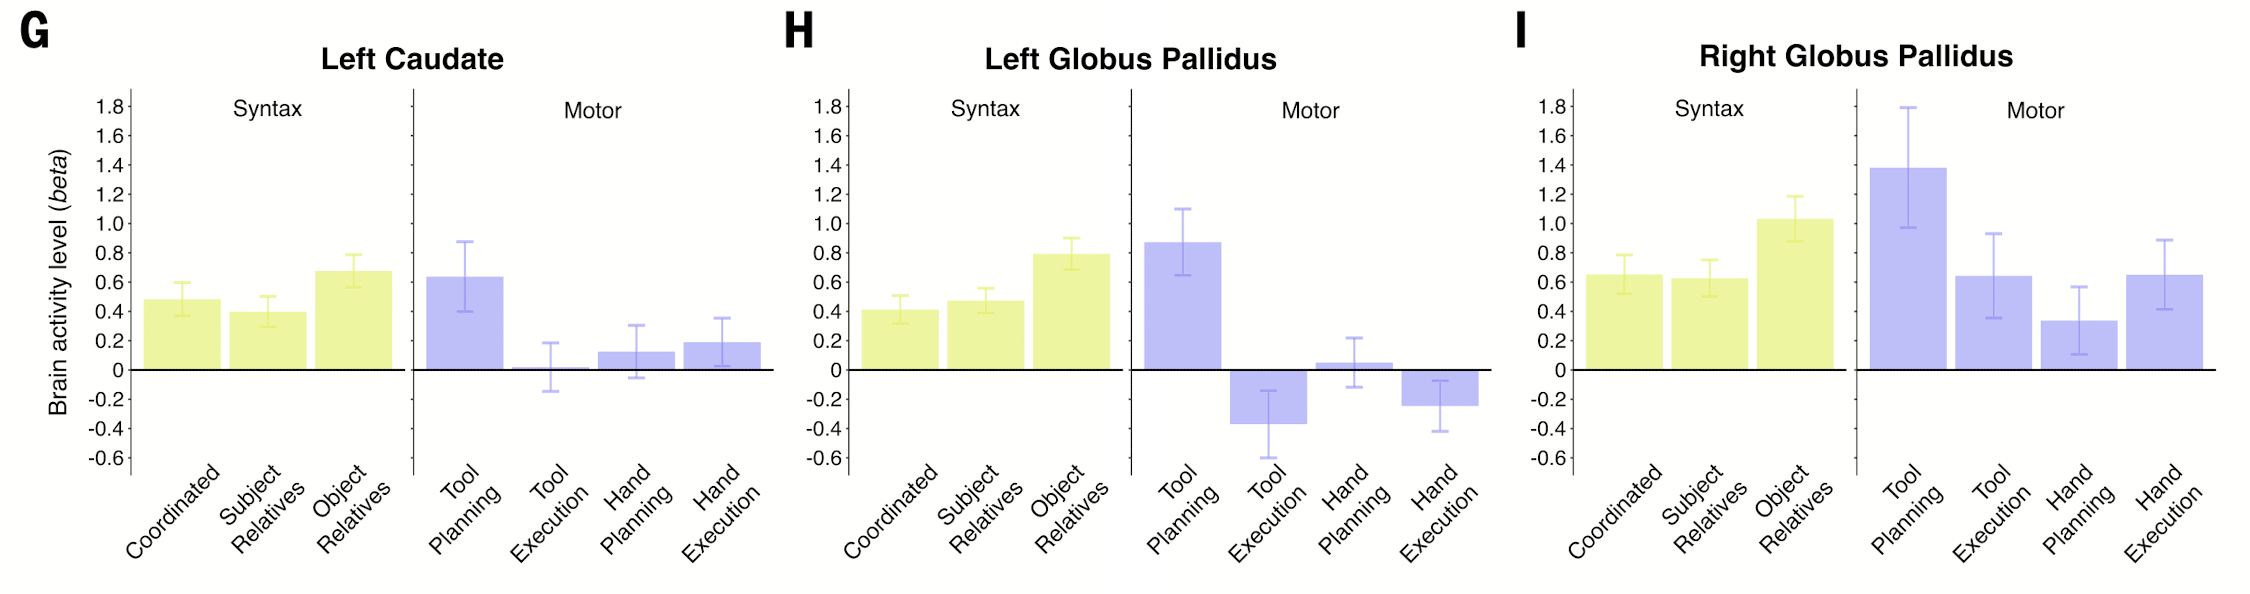
\includegraphics[width=10.5cm]{images/paper_pics/fig1GHI.png}
    \caption*{Syntactic and tool-use planning shared significant activations of the left caudate nucleus (lCau) and bilateral GPi}
    \label{fig:label4}
\end{figure}
}
\pause
\only<2>{
\begin{itemize}
\item Both networks anatomically \textbf{overlapped} within the \textbf{BG}
\item Clusters found in proximity of left IFG did not overlap
\item \textbf{No} significant \textbf{shared} activation for \textbf{syntax} and \textbf{free-hand planning}
\end{itemize}}
\pause

\only<3>{{\large \textbf{To \textbf{rule out} contribution of \textbf{working memory} to this overlap}\\
\begin{itemize}
    \item Measured brain activity while same participants performed two verbal \textbf{n-back tasks}
    \item \textbf{Did not} significantly \textbf{overlap} with tool-use planning network
\end{itemize}}}

\end{frame}

\begin{frame}{Experiment 1}
\setbeamercovered{invisible}
\fontsize{11pt}{15}\selectfont
\textbf{Tool use} and \textbf{syntax} rely on \textbf{neural activity} within common anatomical territories in the BG.\\ %Brain activity displays similar spatial distribution
\begin{figure}
    \centering
    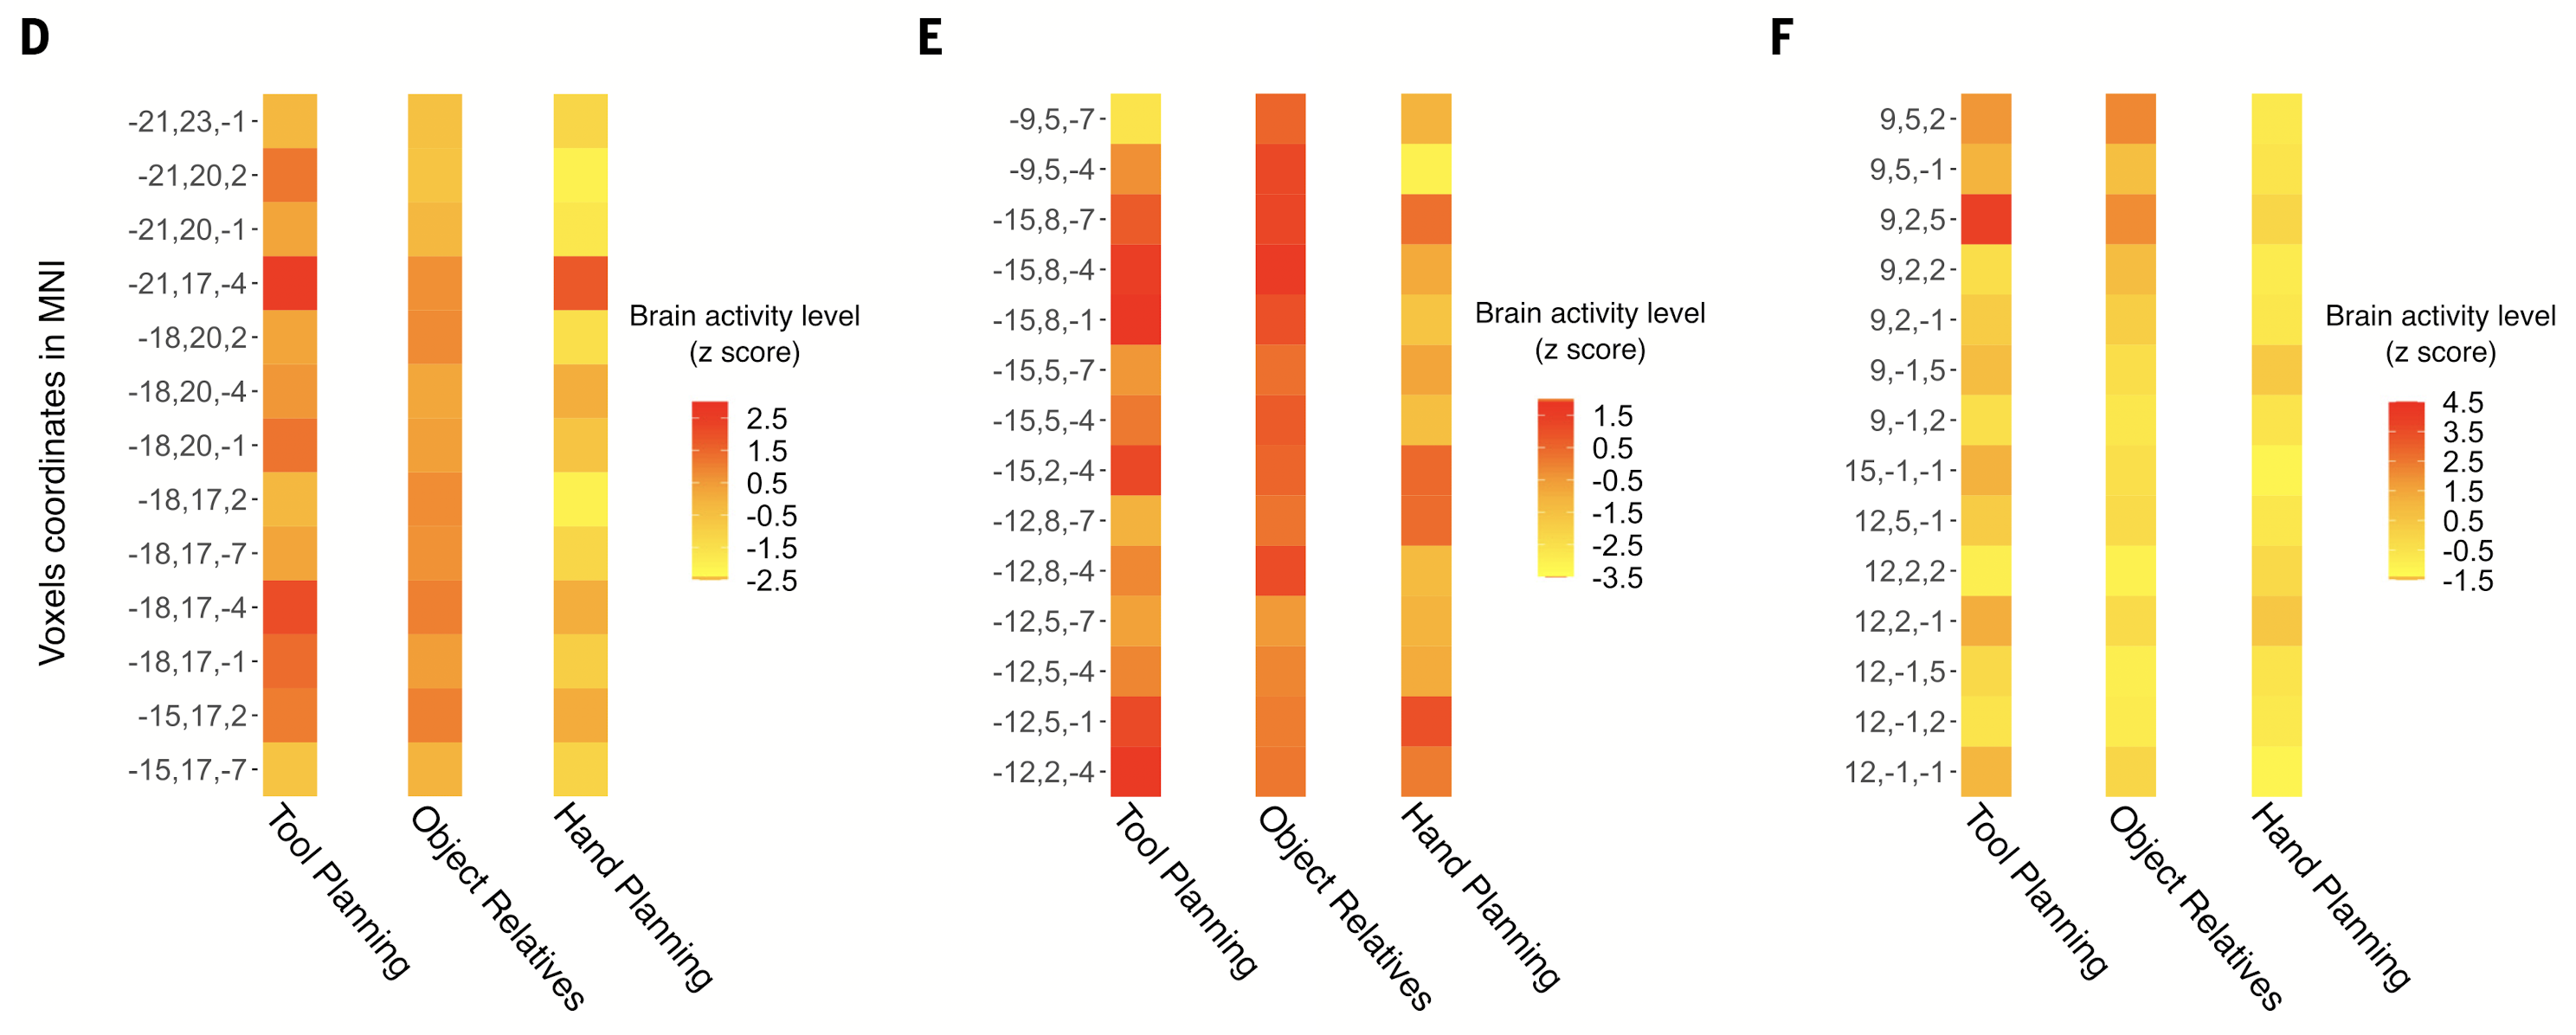
\includegraphics[width=10.5cm]{images/paper_pics/fig2DEF.png}
    \caption*{Spatial distribution of neural activity for tool-use planning, object-relative planning, and free-hand planning in the BG. Each single colored square represents a single voxel for the lCau (D), lGPi (E), and rGPi (F).}
    \label{fig:label5}
\end{figure}

\end{frame}

\section{Experiment 2}

\begin{frame}{Experiment 2}
\setbeamercovered{invisible}
\fontsize{11pt}{15}\selectfont
\only<1>{{\large Previous studies documented that when two functions \textbf{share} neural resources and cognitive processes, \textbf{learning transfer} occurs.}}
\pause
\only<2>{\Large\textbf{Aim:}\\
\vspace{0.2cm}
{\large\textbf{Test whether tool-use training improves syntactic skills in language.}}}
\vspace{0.3cm}
\pause
\only<3>{{\Large \textbf{Experimental design:}}
\begin{itemize}
    \item 3 groups of participants
    \item Same syntactic task as in Experiment 1
    \item Performed before and after some training
\end{itemize}}
\pause
\only<4>{\begin{block*}{}
\footnotesize % Adjust the font size if needed
\begin{columns}[T]
\begin{column}{0.3\textwidth} % Adjusted width for the first column
{\normalsize \textbf{First group:}}
\vspace{0.2cm}
\begin{itemize}
    \item Carried out syntactic task
    \item Training with \textbf{tool}
\end{itemize}
\end{column}
\begin{column}{0.3\textwidth} % Adjusted width for the second column
{\normalsize \textbf{Second group:}}
\vspace{0.2cm}
\begin{itemize}
    \item To control for specificity of tool
    \item Training with \textbf{free hand} 
\end{itemize}
\end{column}
\begin{column}{0.3\textwidth} % Adjusted width for the third column
{\normalsize \textbf{Third group:}}
\vspace{0.2cm}
\begin{itemize}
    \item To control for the training
    \item Before and after watching \textbf{documentary clips}
\end{itemize}
\end{column}
\end{columns}
\end{block*}}
\end{frame}


\begin{frame}{Experiment 2}
\setbeamercovered{invisible}
\fontsize{11pt}{15}\selectfont
\only<1>{
\begin{figure}
    \centering
    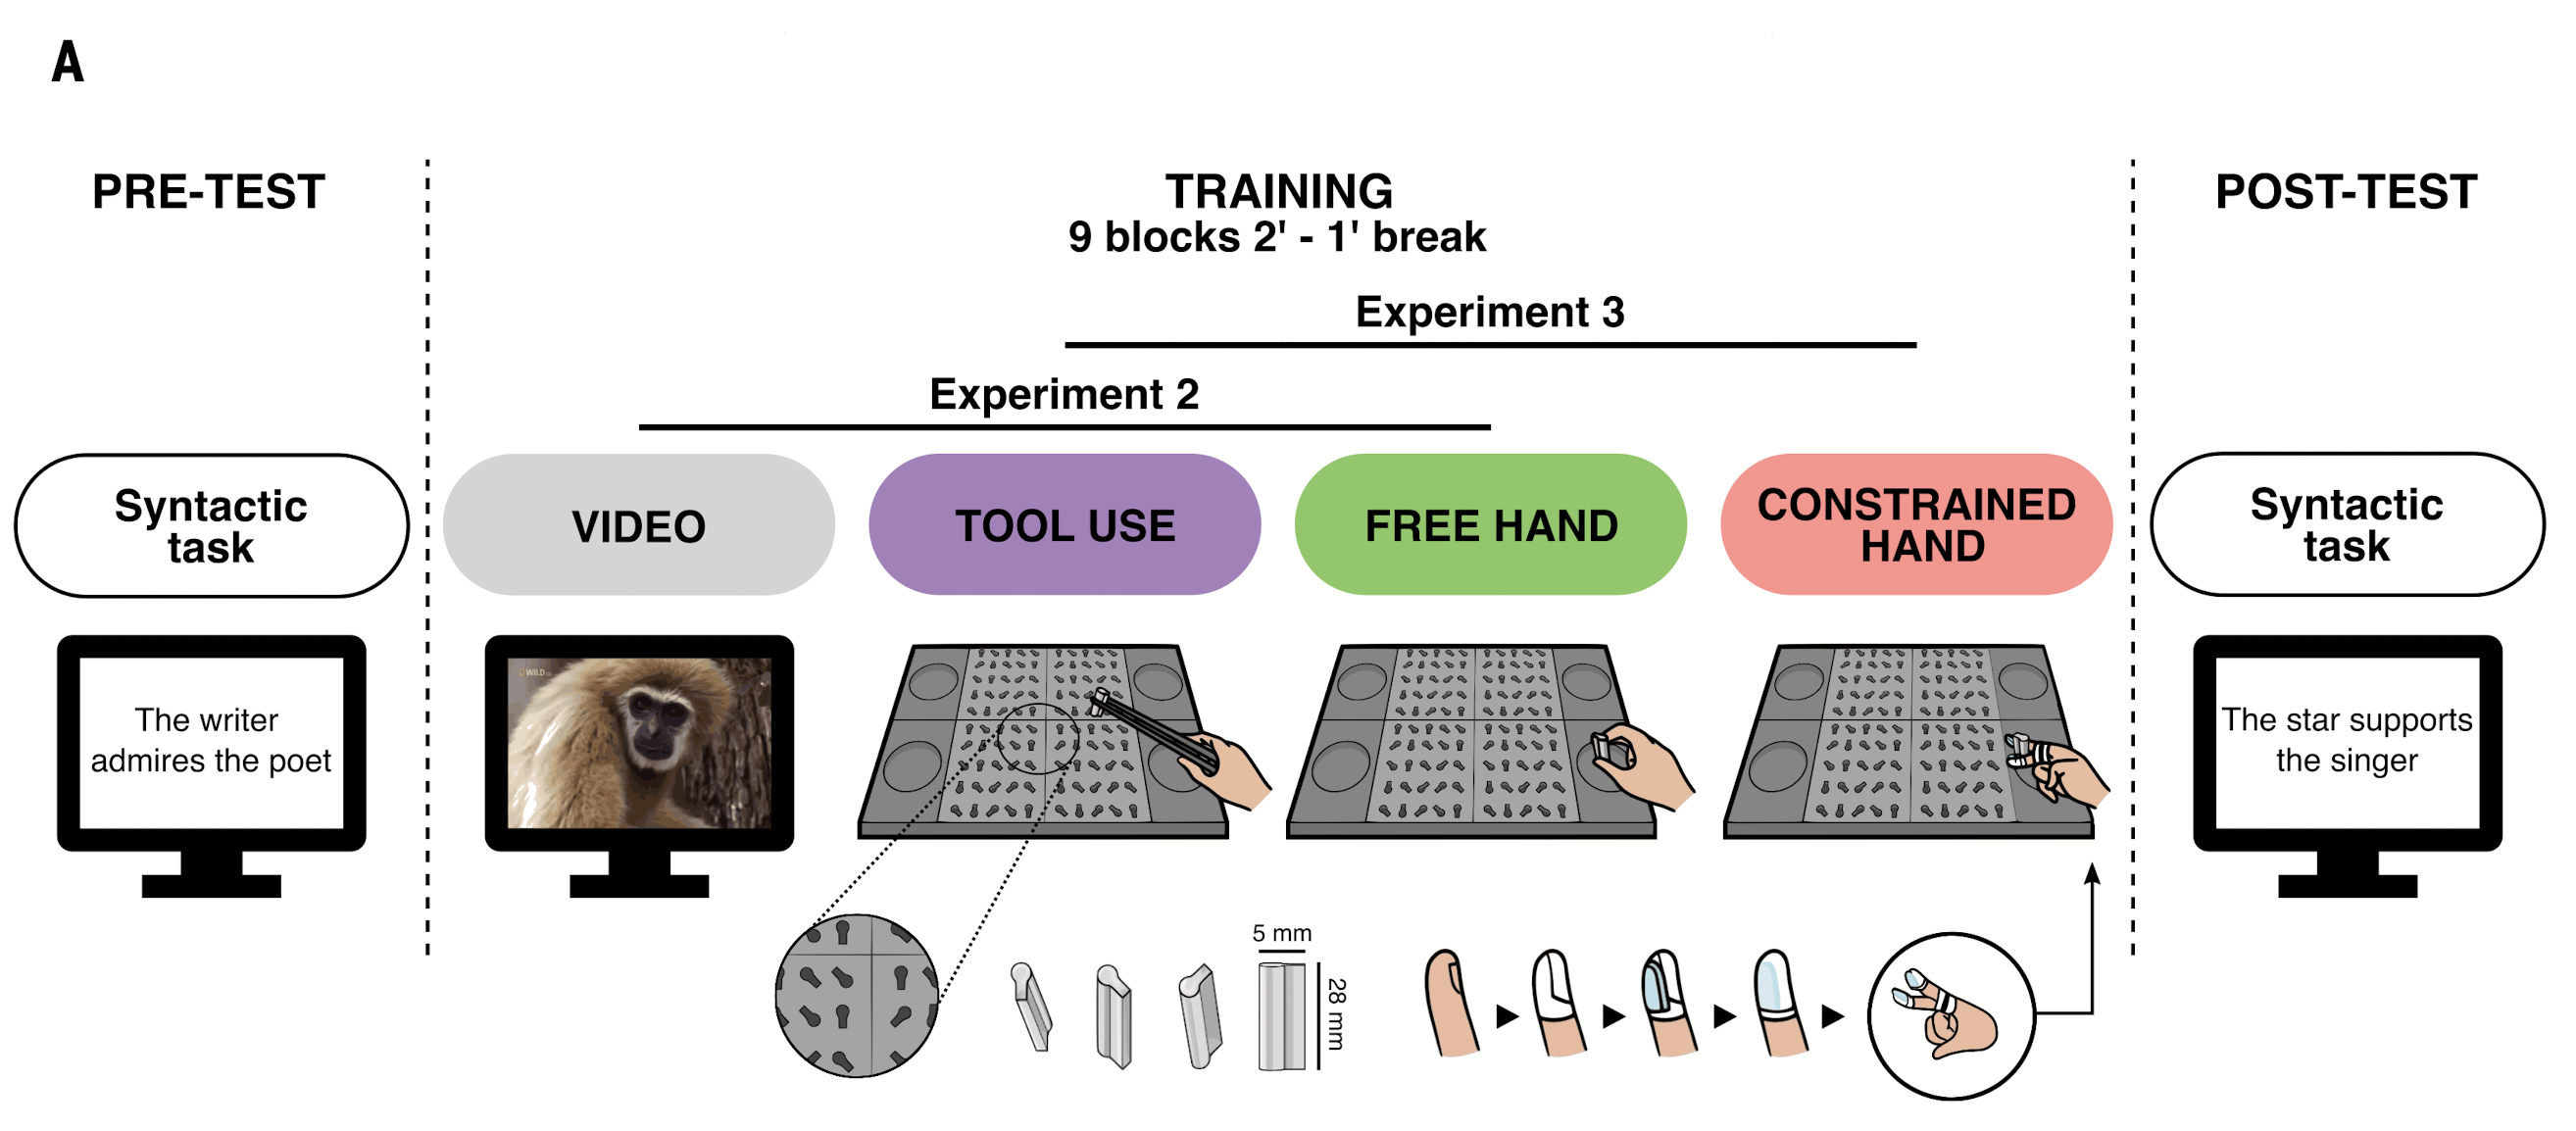
\includegraphics[width=10cm]{images/paper_pics/fig3A.png}
    \caption*{Experiment 2 design}
    \label{fig:label6}
\end{figure}}
\pause
\only<2>{
\begin{figure}
    \centering
    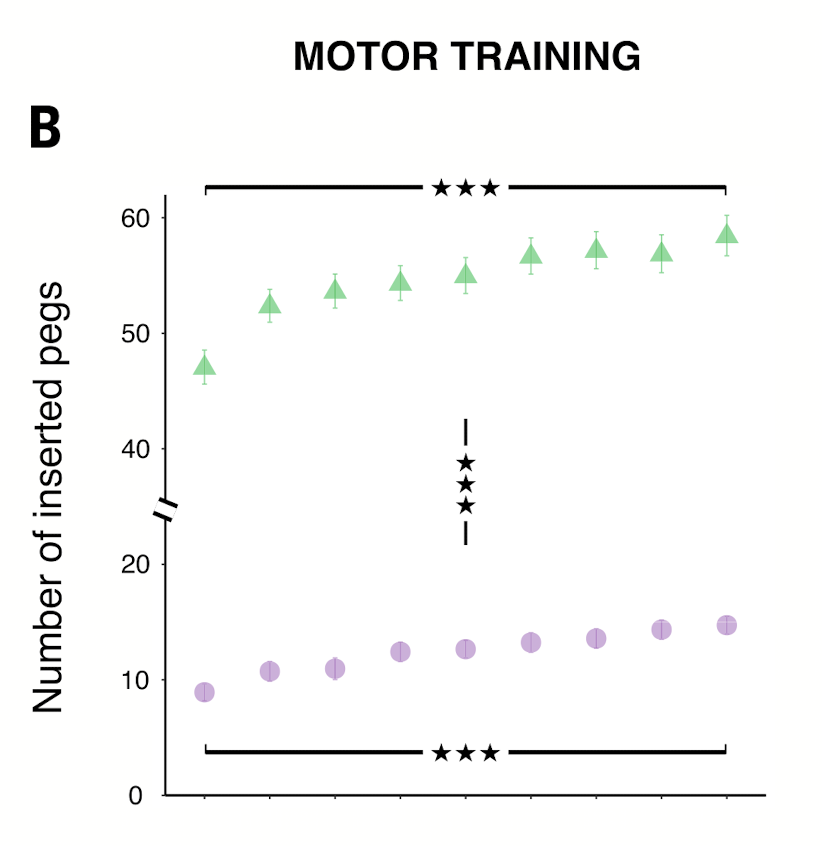
\includegraphics[width=6cm]{images/paper_pics/fig3B.png}
    \caption*{To assess the learning transfer to the syntactic task, they made sure the participants improved in the motor training.}
    \label{fig:label7}
\end{figure}}


\end{frame}

\begin{frame}{Experiment 2}
\setbeamercovered{invisible}
\fontsize{11pt}{15}\selectfont
\only<1>{Analyzed the impact of \textbf{tool-use training} compared with both free-hand training and passive video watching on performance in the syntactic task.}
\pause
\vspace{0.2cm}
\only<2>{{\large\textbf{Results:}}
\begin{itemize}
    \item After \textbf{tool use}, participants were significantly \textbf{faster} in correctly processing object relatives. 
    \item Performance for object relatives \textbf{did not} significantly change for the two \textbf{control groups}.
    \item A significant improvement was found for \textbf{simpler syntactic structures}.
    \item Nevertheless, they were \textbf{equivalent} among the three groups
\end{itemize}}
\pause
\only<3>{{\large\textbf{In a nutshell:}}
\begin{itemize}
    \item Training to use a tool \textbf{improved} syntactic abilities in a linguistic task. 
    \item Depended on the individuals’ initial syntactic level $\rightarrow$ those showing \textbf{better syntactic skills} before training.
\end{itemize}
}

\end{frame}

\section{Experiment 3}

\begin{frame}{Experiment 3}
\setbeamercovered{invisible}
\fontsize{11pt}{15}\selectfont
\vspace{-0.2cm}
\only<1>{{\large\textbf{To confirm those findings, they performed another experiment:\\}}}
\vspace{0.4cm}
\only<1>{{\large\textbf{Experimental design:}}
\begin{itemize}
    \item Three groups of participants with \textbf{high syntactic scores}
    \item Rule out sensorimotor difficulty $\rightarrow$ one group had their \textbf{hand constrained}, mimicking the tool
    \item Syntactic skills were measured in the three groups before and after training
\end{itemize}}
\pause
\only<2>{\begin{block*}{}
\footnotesize
\begin{columns}[T]
\begin{column}{0.3\textwidth}
{\normalsize \textbf{First group:}}
\vspace{0.2cm}
\begin{itemize}
    \item Carried out syntactic task
    \item Training with \textbf{tool}
\end{itemize}
\end{column}
\begin{column}{0.3\textwidth}
{\normalsize \textbf{Second group:}}
\vspace{0.2cm}
\begin{itemize}
    \item To control for specificity of tool
    \item Training with \textbf{free hand} 
\end{itemize}
\end{column}
\begin{column}{0.3\textwidth}
{\normalsize \textbf{Third group:}}
\vspace{0.2cm}
\begin{itemize}
    \item To control for the sensorimotor difficulty
    \item Training with \textbf{constrained hand}
\end{itemize}
\end{column}
\end{columns}
\end{block*}}

\end{frame}

\begin{frame}{Experiment 3}
\setbeamercovered{invisible}
\fontsize{11pt}{15}\selectfont


\only<1>{
\begin{figure}
    \centering
    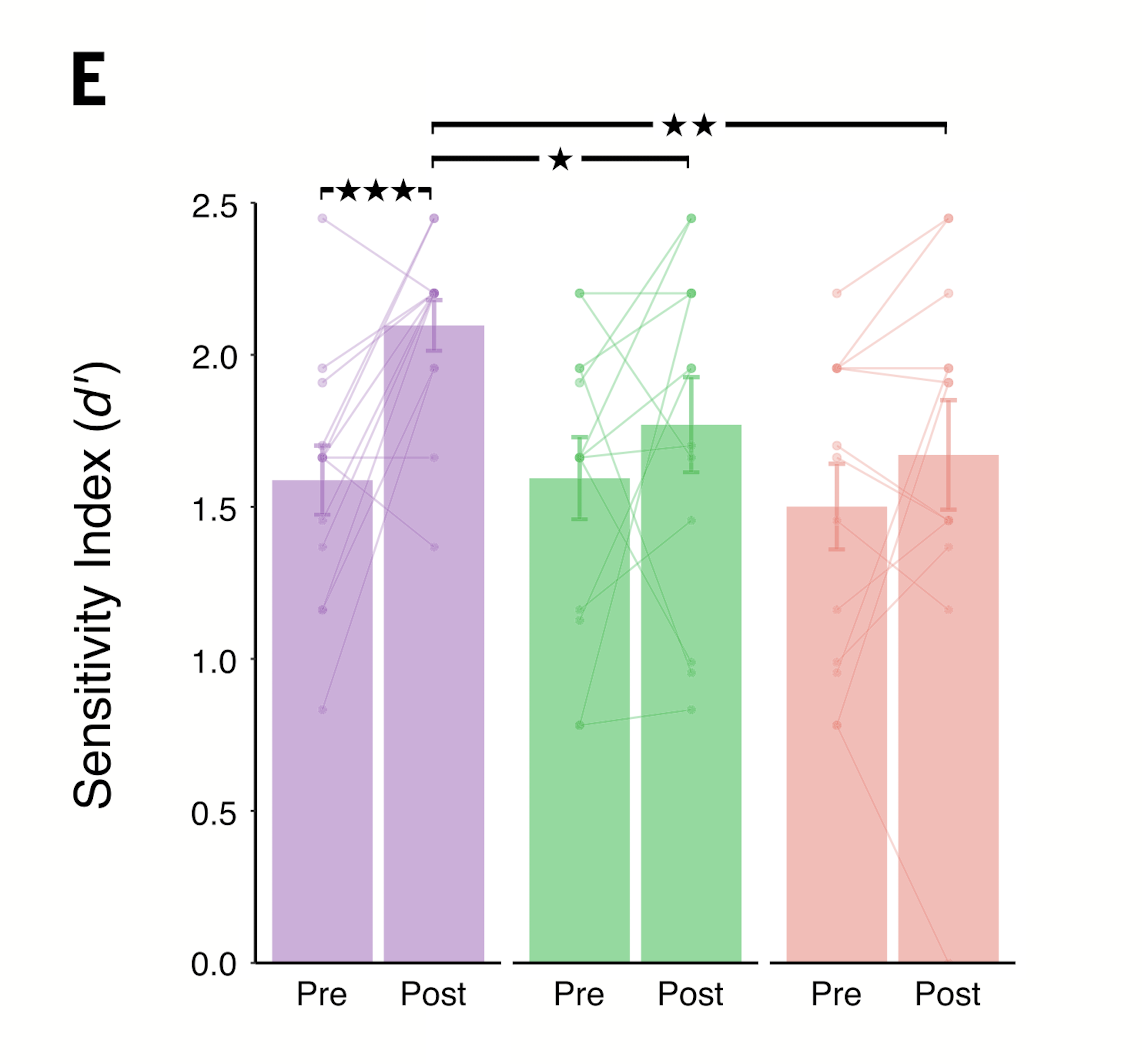
\includegraphics[width=6.5cm]{images/paper_pics/fig3E.png}
    \caption*{Participants improved for \textbf{object relatives} in the syntactic task (purple), but not after training with the free hand (green) or with the constrained hand (red)}
    \label{fig:label9}
\end{figure}
}

\pause
\only<2>{
{\large\textbf{Results:}}
\begin{itemize}
    \item Reconfirmed that \textbf{tool-use training} selectively \textbf{improved} comprehension of object relatives
    \item \textbf{Neither} free-hand training nor constrained-hand training significantly \textbf{enhanced} the performance for object relatives
    \item \textbf{After training}, the tool-use group significantly \textbf{outperformed} the others on object relatives comprehension
\end{itemize}
}

\end{frame}


%\section{Experiment 4}

%\begin{frame}{Experiment 4}
\setbeamercovered{invisible}
\fontsize{12pt}{15}\selectfont
\only<1>{{\large\textbf{Learning transfer from syntactic training in language to tool use}}\\
Testing the \textbf{reverse learning transfer}: training syntactic processes with complex sentences should \textbf{improve tool use}.}
\pause

\only<2>{{\large\textbf{Experimental design:}}
\begin{itemize}
    \item Measuring \textbf{tool-use performance} after syntactic training.
    \item Type of training \textbf{clause} was \textbf{randomly assigned} (unknown to experimenter).
    \item Before and after training, they \textbf{calculated the number of pegs} entered with the tool.
\end{itemize}}
\pause
\only<3>{
\begin{figure}
    \centering
    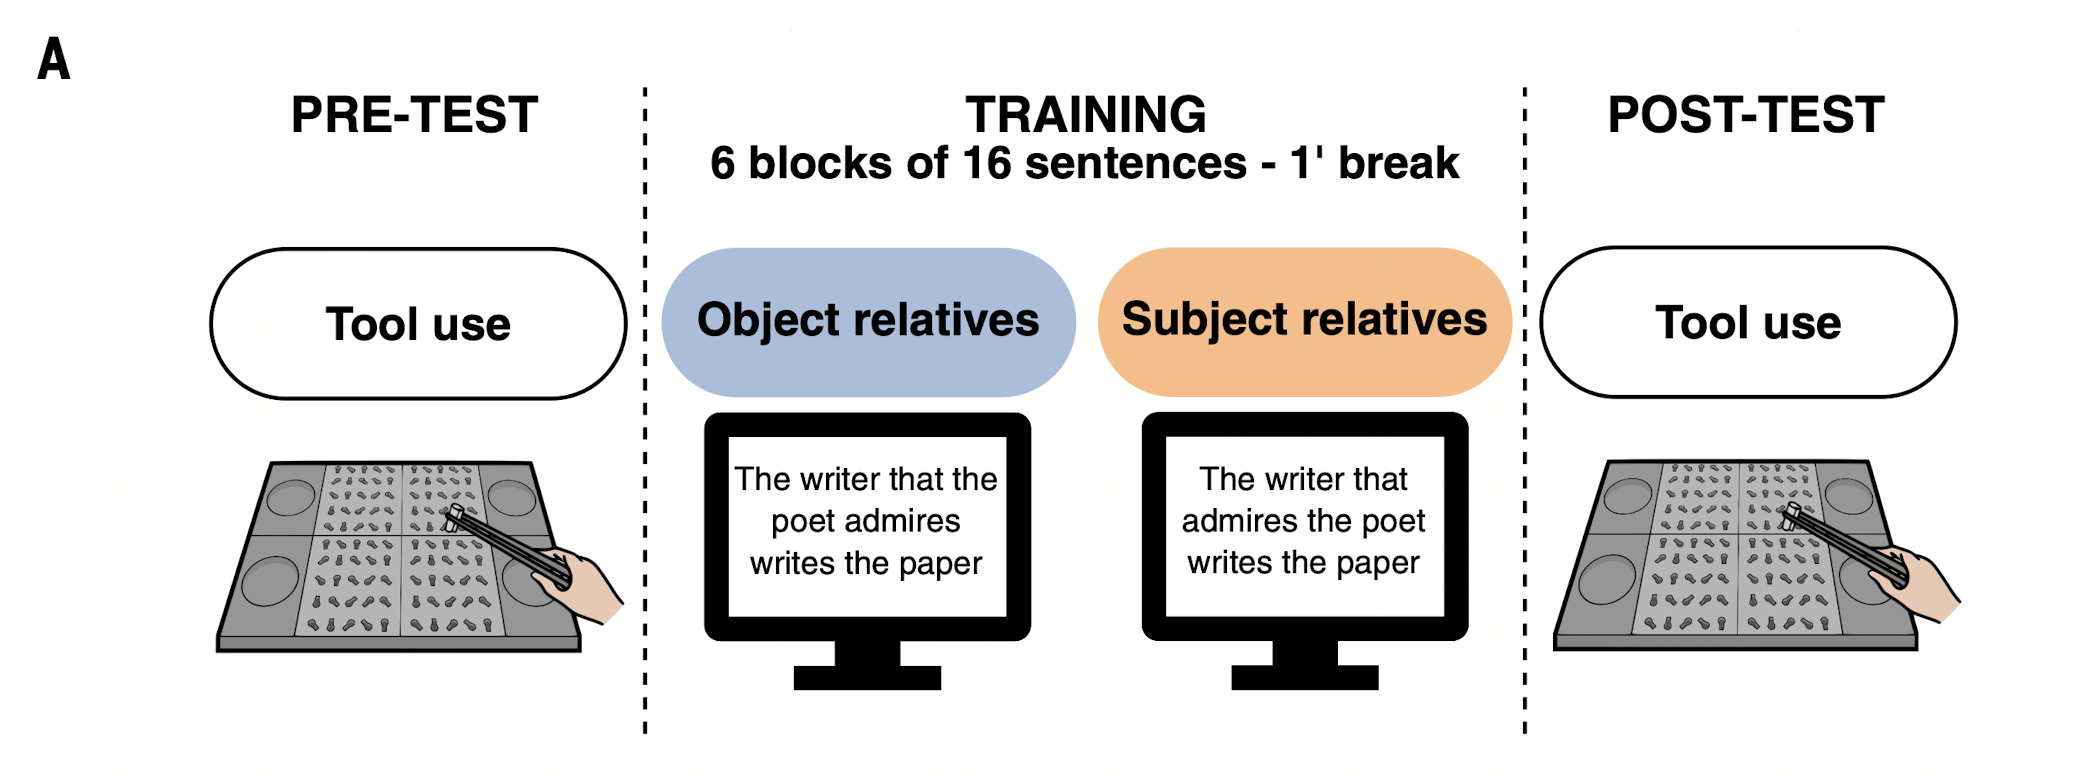
\includegraphics[width=11cm]{images/paper_pics/fig4A.png}
    %\caption*{}
    \label{fig:label10}
\end{figure}
}

\end{frame}


%\begin{frame}{Experiment 4}
\setbeamercovered{invisible}
\fontsize{11pt}{15}\selectfont
\vspace{-0.5cm}
\only<2-4>{\large\textbf{Results:\\}}
\only<1>{{\large Expected the participants to \textbf{perform better} with the tool after \textbf{training with object relatives} rather than with subject relatives.}}
\pause
\only<2>{
\vspace{-0.6cm}
\begin{columns}
    \begin{column}{0.5\textwidth}
    \vspace{-0.3cm}
    \begin{figure}
    \centering
    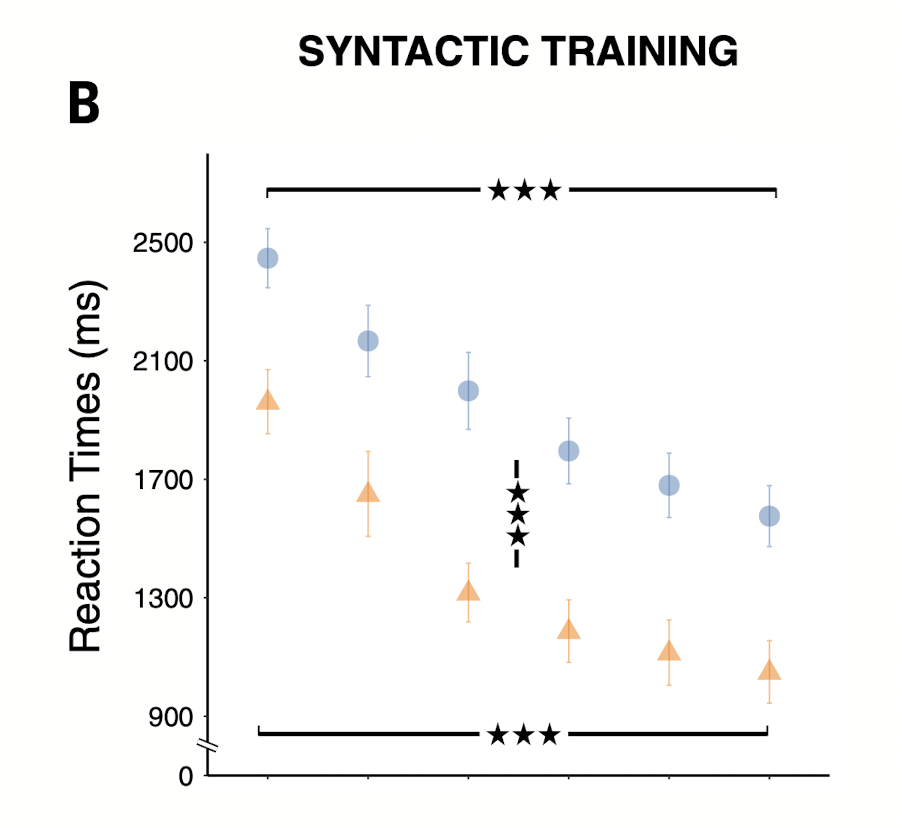
\includegraphics[width=5.6cm]{images/paper_pics/fig4B.png}
    %\caption*{}
    \label{fig:label11}
\end{figure}
    \end{column}
    \begin{column}{0.5\textwidth}
    \vspace{0.7cm}
        \begin{figure}
    \centering
    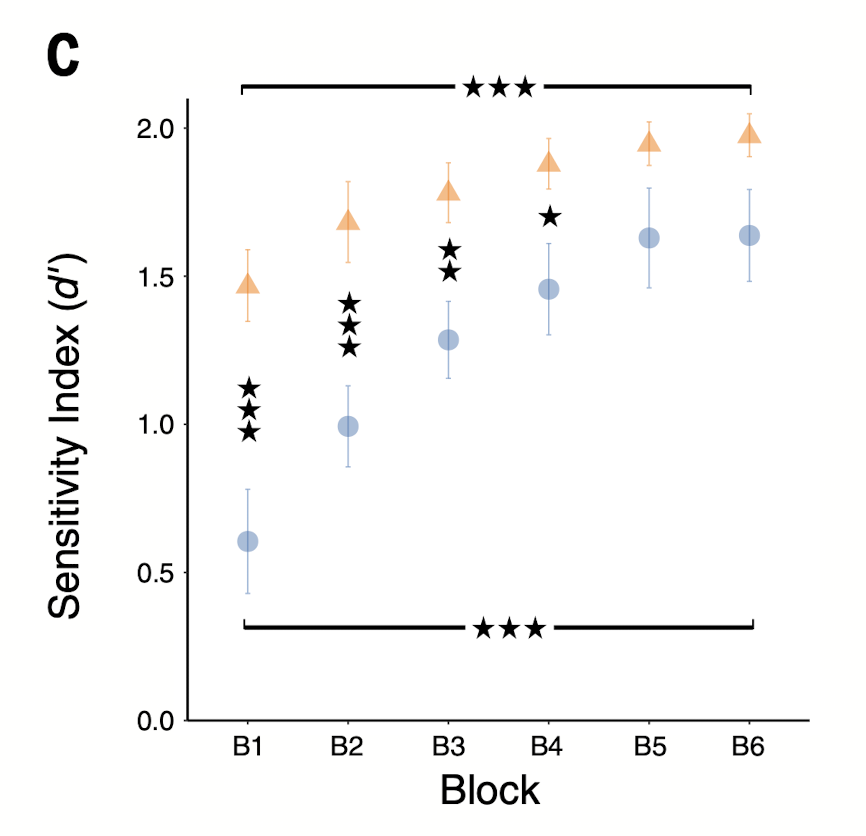
\includegraphics[width=5.6cm]{images/paper_pics/fig4C.png}
    %\caption*{}
    \label{fig:label12}
\end{figure}
    \end{column}
\end{columns}
\vspace{-0.7cm}
\hspace{1cm}{\footnotesize Both groups improved in processing relative sentences during training.}
}
\pause
\only<3>{
\begin{figure}
    \centering
    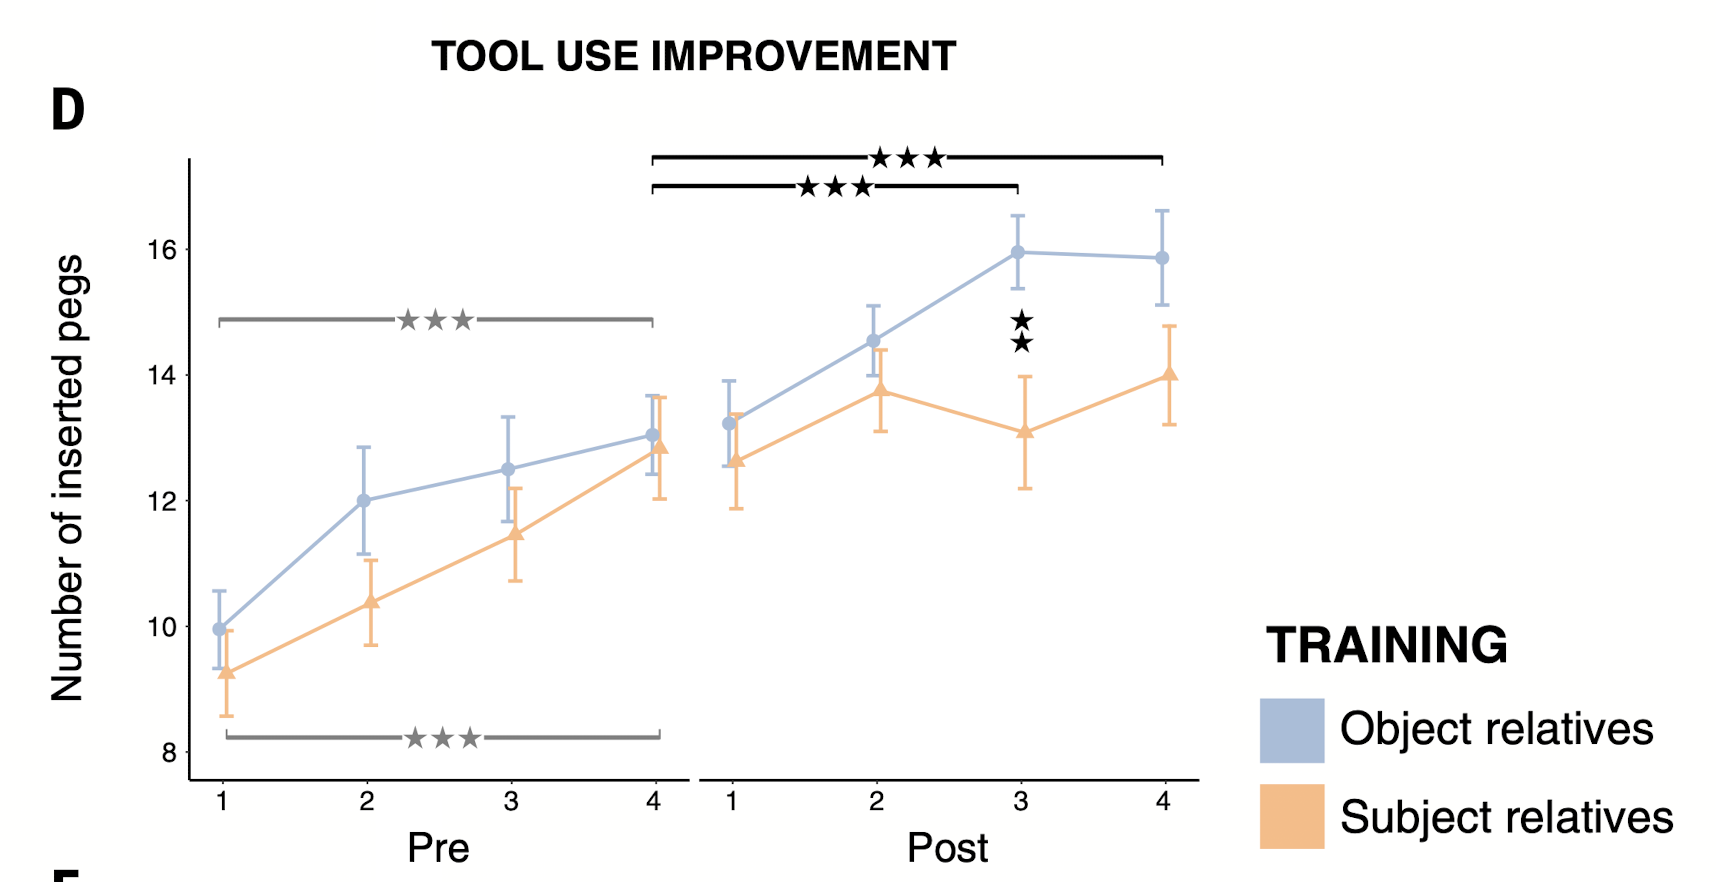
\includegraphics[width=10cm]{images/paper_pics/fig4D.png}
    \vspace{0.2cm}
    \caption*{{\footnotesize Participants who trained with \textbf{object relatives} kept improving significantly with the tool.}}
    \label{fig:label12}
    \end{figure}
    }

\only<4>{
\begin{itemize}
\vspace{0.2cm}
    \item Training with subject relatives did not change participants’ motor performance.
\end{itemize}
    
}


\end{frame}

%\section{Experiment 5}

%\begin{frame}{Experiment 5}
\setbeamercovered{invisible}
\fontsize{11pt}{15}\selectfont
\only<1>{\begin{figure}
    \centering
    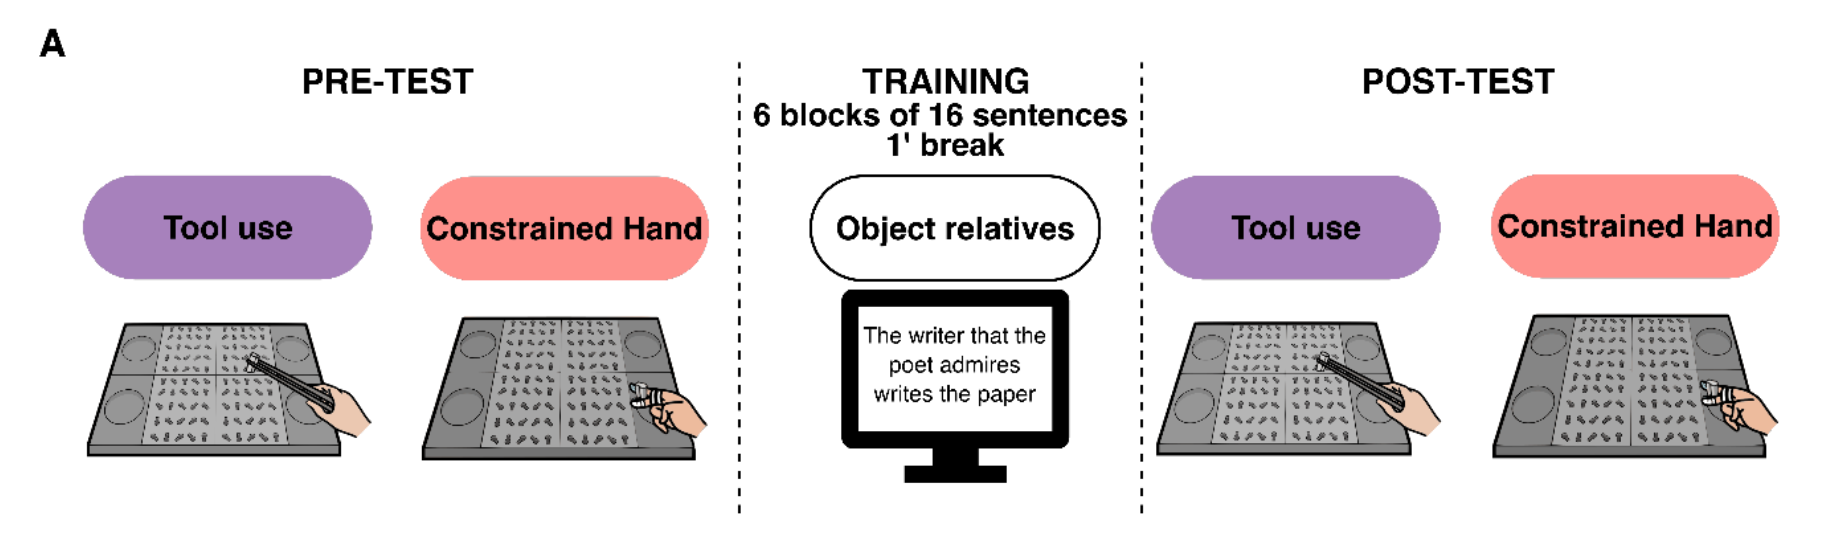
\includegraphics[width=9cm]{images/paper_pics/figS4A.png}
    \caption*{Two groups were tested in entering pegs as fast as possible with the tool (purple) or the constrained hand (red), before and after training with object relative clauses.}
    \label{fig:label12}
\end{figure}}
\pause
\only<2>{{\large\textbf{Results:\\}}
\begin{itemize}
    \item Motor improvement observed after linguistic training with object relatives is \textbf{specific} to \textbf{tool use}.
    \item \textbf{After training}, participants inserted \textbf{more pegs with the tool} than the constrained hand.
\end{itemize}
}



\end{frame}

\section{Discussion}

\begin{frame}{Discussion}
\setbeamercovered{invisible}
\fontsize{12pt}{16}\selectfont

\only<1>{\begin{itemize}
\item Tool use and syntax rely on brain activity of \textbf{anatomically overlapping} neural networks, particularly in striatal structures (lCau) and the GPi.
\item Working memory processes were not involved.
\end{itemize}}
\pause
\vspace{-0.2cm}
\only<2-3>{{\large\textbf{These findings:\\}}
\begin{itemize}
    \only<2>{\item Support the hypothesis of a \textbf{supramodal syntactic function} serving both domains
    \item \textbf{Consistent} with studies claiming role of the \textbf{dorsal striatum} in \textbf{processing complex hierarchical structures} in both the motor and linguistic domains.
    \item This area is involved in \textbf{syntactic training} and in the implementation of grammatical rules.
    \item It works as a \textbf{parser} of actions to chunk motor sequences}
    \pause
    \only<3>{\item Accurate and efficient tool use requires \textbf{embedding} an \textbf{external object} into the motor sequence and thus relies more on the striatum than on manual actions to parse the motor primitives
    \item \textbf{Parsing} and \textbf{hierarchy} handling also support syntactic comprehension of \textbf{center-embedded object relatives}
    \item These functional similarities are reflected by the neural overlap.}
\end{itemize}
}

\only<4>{\textbf{However,}\\
\begin{itemize}
    \item The complexity of the hierarchies to be handled might not be strictly proportionate [no further elaboration]
    \item \textbf{Overlap} was found in the \textbf{BG} but not in the left IFG
\end{itemize}
}


\end{frame}

%\begin{frame}{Discussion}
\setbeamercovered{invisible}
\fontsize{12pt}{16}\selectfont
%\vspace{-0.4cm}


\only<1>{
\begin{itemize}
\item Results explain the \textbf{cross-domain learning transfer} from tool use to syntactic skills in language and viceversa.
\item Learning transfer happens only if trained and untrained tasks rely on \textbf{overlapping neural networks} and \textbf{shared cognitive processes}.
\item Transfer effects had been demonstrated so far only in the same domain: perception, motor, or cognitive control.
\end{itemize}}
\pause
\only<2>{
\begin{itemize}
\item Transfer \textbf{holds true} even when different cognitive domains are involved.
\item Transfer might be absent if trained and untrained tasks do not share common neurocognitive resources.
\end{itemize}}
\pause
\only<3>{
\begin{itemize}
\item Training with subject-relative structures did not improve motor performance with the tool.
\item \textbf{Free-hand} training \textbf{failed} to induce benefits to syntax in the comprehension of complex structures.
\end{itemize}}

\pause
\only<4>{
\begin{itemize}
    \item \textbf{Benefits} induced by tool use over language were \textbf{not based} on the mere \textbf{additional sensorimotor complexity} of the action executed with the tool compared with the free hand.
    \item After training with a \textbf{constrained hand}, the participants did not show \textbf{any advantage} in processing complex syntactic structures.
\end{itemize}}
\pause
\only<5>{
\begin{itemize}
    \item The learning \textbf{transfer} between tool use and syntactic processes in language occurs \textbf{bidirectionally}.
    \item Unambiguously indicates that the two abilities rely on a common cognitive component, namely a \textbf{supramodal syntax}.
\end{itemize}}

\end{frame}

%\begin{frame}{Discussion}
\setbeamercovered{invisible}
\fontsize{12pt}{16}\selectfont
\only<1>{\begin{itemize}
\item Reignite the hypothesis of a \textbf{coevolution} of tool use and language
\item The \textbf{birth} and \textbf{refinement} of tool use may have offered the \textbf{neural habitat} for the coevolution of both motor and communicative skills.
\end{itemize}}
\pause
\only<2>{\begin{columns}
\hspace{-0.1cm}
\vspace{0.2cm}
    \begin{column}{0.5\textwidth}
        The \textbf{sophistication of tool use} and tool \textbf{making} has put forward the need for cognitive functions to \textbf{efficiently chunk}, temporally \textbf{parse}, and deal with \textbf{hierarchies} of sequences.
    \end{column}
    \begin{column}{0.5\textwidth}
        Tool use and tool making posed \textbf{evolutionary pressure} for communication, allowing better \textbf{social transmission} of knowledge.
    \end{column}
\end{columns}}
\pause
\only<3>{
\begin{itemize}

\item So functions initially serving the motor system would have \textbf{adapted and repurposed} for language and communication.

\item $\rightarrow$ This coevolution scenario has involved a \textbf{broad brain network}: spanning from parietal to frontal regions, including the BG.
\end{itemize}}


\end{frame}

\begin{frame}{Discussion}
\setbeamercovered{invisible}
\fontsize{12pt}{16}\selectfont

{\large \textbf{In conclusion:\\}}
\begin{itemize}
\item Provide evidence pointing to the \textbf{BG} in particular as the neural \textbf{niche for a supramodal syntactic function} serving both action and language. 
\item Show that the \textbf{motor system} can be exploited to promote \textbf{other cognitive functions} that partly share the same neurocognitive foundations.
\end{itemize}

%\begin{figure}
%    \centering
%    \includegraphics[width=7cm]{images/paper_pics/fig6.jpeg}
%    \caption*{Sublinear fashion}
%    \label{fig:label78}
%\end{figure}

\end{frame}

%\cventry{}{\vspace*{-1.2\baselineskip}\printbibliography}{}{}{}{}

%\vspace{2cm}{\printbibliography[title={Bibliography}]}
\end{document}
